\documentclass[tikz,border=8pt]{standalone}
\usetikzlibrary{automata,positioning,arrows.meta}
\begin{document}
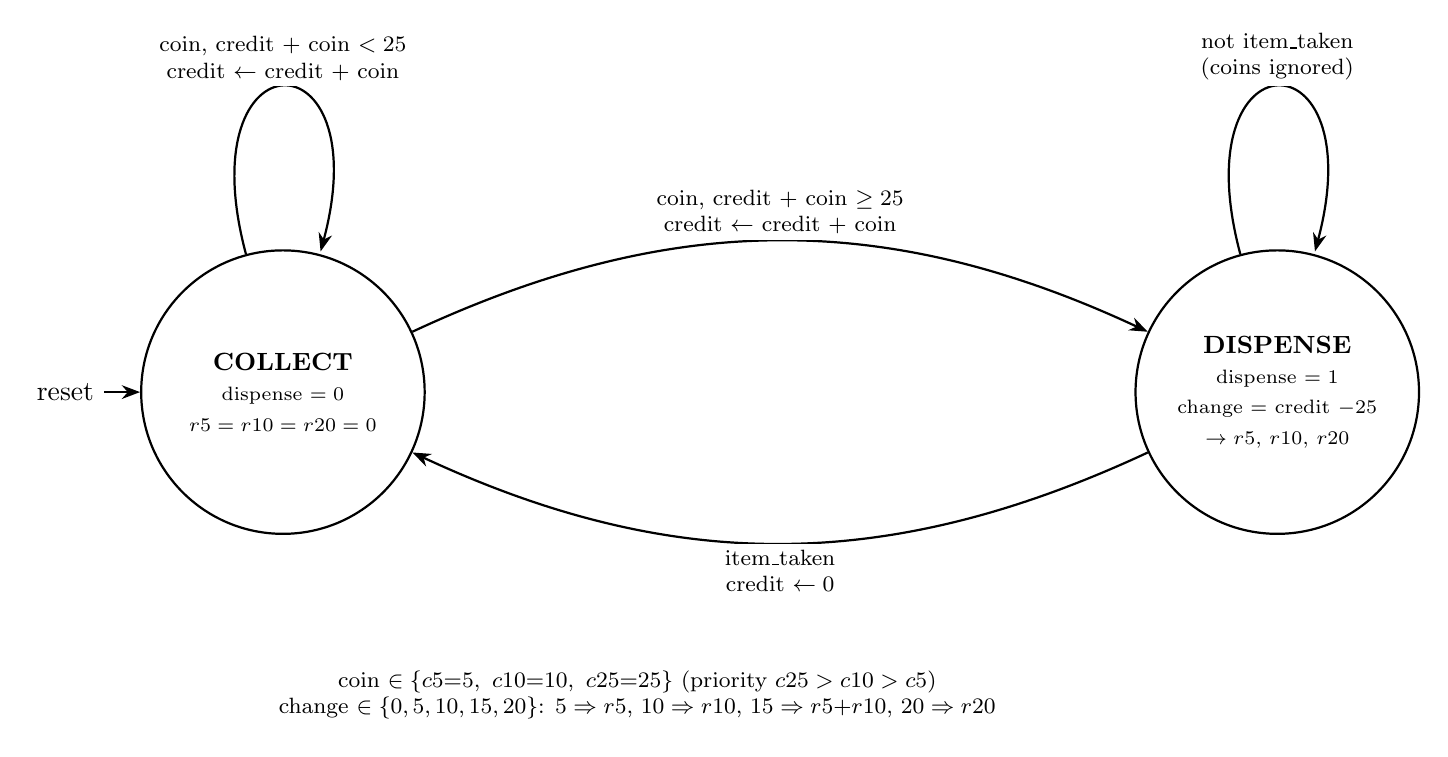
\begin{tikzpicture}[>=Stealth, node distance=9cm, auto,
  every state/.style={draw, thick, minimum size=3.6cm, align=center, font=\small},
  every edge/.style={draw, thick, ->},
  lbl/.style={font=\footnotesize, align=center, fill=white, inner sep=2pt}]

  \node[state, initial, initial text=reset] (C)
    {\textbf{COLLECT}\\ \scriptsize dispense $=0$\\ \scriptsize $r5=r10=r20=0$};
  \node[state, right=of C] (D)
    {\textbf{DISPENSE}\\ \scriptsize dispense $=1$\\ \scriptsize change $=$ credit $-25$\\ \scriptsize $\rightarrow r5,\,r10,\,r20$};

  \path (C) edge[loop above] node[lbl]{coin, credit $+$ coin $<25$\\ credit $\leftarrow$ credit $+$ coin} (C)
        (C) edge[bend left=25] node[lbl]{coin, credit $+$ coin $\ge 25$\\ credit $\leftarrow$ credit $+$ coin} (D)
        (D) edge[bend left=25] node[lbl]{item\_taken\\ credit $\leftarrow 0$} (C)
        (D) edge[loop above] node[lbl]{not item\_taken\\ (coins ignored)} (D);

  \node[font=\footnotesize, align=center, below=1.6cm of C, xshift=4.5cm]
    {coin $\in\{c5{=}5,\ c10{=}10,\ c25{=}25\}$ (priority $c25>c10>c5$)\\
     change $\in\{0,5,10,15,20\}$: $5\Rightarrow r5$, $10\Rightarrow r10$, $15\Rightarrow r5{+}r10$, $20\Rightarrow r20$};
\end{tikzpicture}
\end{document}
